% Preámbulo
\documentclass[letterpaper]{article}
\usepackage[utf8]{inputenc}
\usepackage[spanish]{babel}
\decimalpoint

\usepackage{enumitem}
\usepackage{titling}

% Símbolos
	\usepackage{amsmath}
	\usepackage{amssymb}
	\usepackage{amsthm}
	\usepackage{amsfonts}
	\usepackage{mathtools}
	\usepackage{bbm}
	\usepackage[thinc]{esdiff}
	\allowdisplaybreaks

% Márgenes
	\usepackage
	[
		margin = 1.2in
	]
	{geometry}

% Imágenes
	\usepackage{float}
	\usepackage{graphicx}
	\graphicspath{{imagenes/}}
	\usepackage{subcaption}

% Ambientes
	\usepackage{amsthm}

	\theoremstyle{definition}
	\newtheorem{ejercicio}{Ejercicio}

	\newtheoremstyle{lemathm}{4pt}{0pt}{\itshape}{0pt}{\bfseries}{ --}{ }{\thmname{#1}\thmnumber{ #2}\thmnote{ (#3)}}
	\theoremstyle{lemathm}
	\newtheorem{lema}{Lema}

	\newtheoremstyle{lemathm}{4pt}{0pt}{\itshape}{0pt}{\bfseries}{ --}{ }{\thmname{#1}\thmnumber{ #2}\thmnote{ (#3)}}
	\theoremstyle{lemathm}
	\newtheorem{sol}{Solución}
	
	\newtheoremstyle{lemathm}{4pt}{0pt}{\itshape}{0pt}{\bfseries}{ --}{ }{\thmname{#1}\thmnumber{ #2}\thmnote{ (#3)}}
	\theoremstyle{lemathm}
	\newtheorem{theo}{Teorema}

	\newtheoremstyle{lemademthm}{0pt}{10pt}{\itshape}{ }{\mdseries}{ --}{ }{\thmname{#1}\thmnumber{ #2}\thmnote{ (#3)}}
	\theoremstyle{lemademthm}
	\newtheorem*{lemadem}{Demostración}

% Macros
	\newcommand{\sumi}[2]{\sum_{i=#1}^{#2}}
	\newcommand{\dint}[2]{\displaystyle\int_{#1}^{#2}}
	\newcommand{\inte}[2]{\int_{#1}^{#2}}
	\newcommand{\dlim}{\displaystyle\lim}
	\newcommand{\limxinf}{\lim_{x\to\infty}}
	\newcommand{\limninf}{\lim_{n\to\infty}}
	\newcommand{\dlimninf}{\displaystyle\lim_{n\to\infty}}
	\newcommand{\limh}{\lim_{h\to0}}
	\newcommand{\ddx}{\dfrac{d}{dx}}
	\newcommand{\txty}{\text{ y }}
	\newcommand{\txto}{\text{ o }}
	\newcommand{\Txty}{\quad\text{y}\quad}
	\newcommand{\Txto}{\quad\text{o}\quad}
	\newcommand{\si}{\text{si}\quad}

	\newcommand{\etiqueta}{\stepcounter{equation}\tag{\theequation}}
	\newcommand{\tq}{:}
	\renewcommand{\o}{\circ}
	\newcommand*{\QES}{\hfill\ensuremath{\blacksquare}}
	\newcommand*{\qes}{\hfill\ensuremath{\square}}
	\newcommand*{\QESHERE}{\tag*{$\blacksquare$}}
	\newcommand*{\qeshere}{\tag*{$\square$}}
	\newcommand*{\QED}{\hfill\ensuremath{\blacksquare}}
	\newcommand*{\QEDHERE}{\tag*{$\blacksquare$}}
	\newcommand*{\qel}{\hfill\ensuremath{\boxdot}}
	\newcommand*{\qelhere}{\tag*{$\boxdot$}}
	\renewcommand*{\qedhere}{\tag*{$\square$}}

	\newcommand{\suc}[1]{\left(#1_n\right)_{n\in\N}}
	\newcommand{\en}[2]{\binom{#1}{#2}}
	\newcommand{\upsum}[2]{U(#1,#2)}
	\newcommand{\lowsum}[2]{L(#1,#2)}
	\newcommand{\abs}[1]{\left| #1 \right| }
	\newcommand{\bars}[1]{\left \| #1 \right \| }
	\newcommand{\pars}[1]{\left( #1 \right) }
	\newcommand{\bracs}[1]{\left[ #1 \right] }
	\newcommand{\inprod}[1]{\left\langle #1 \right\rangle }
    \newcommand{\norm}[1]{\left\lVert#1\right\rVert}
	\newcommand{\floor}[1]{\left \lfloor #1 \right\rfloor }
	\newcommand{\ceil}[1]{\left \lceil #1 \right\rceil }
	\newcommand{\angles}[1]{\left \langle #1 \right\rangle }
	\newcommand{\set}[1]{\left \{ #1 \right\} }
	\newcommand{\norma}[2]{\left\| #1 \right\|_{#2} }


	\newcommand{\NN}{\mathbb{N}}
	\newcommand{\QQ}{\mathbb{Q}}
	\newcommand{\RR}{\mathbb{R}}
	\newcommand{\ZZ}{\mathbb{Z}}
	\newcommand{\PP}{\mathbb{P}}
    \newcommand{\EE}{\mathbb{E}}
	\newcommand{\1}{\mathbbm{1}}
	\newcommand{\eps}{\varepsilon}
	\newcommand{\ttF}{\mathtt{F}}
	\newcommand{\bfF}{\mathbf{F}}

	\newcommand{\To}{\longrightarrow}
	\newcommand{\mTo}{\longmapsto}
	\newcommand{\ssi}{\Longleftrightarrow}
	\newcommand{\sii}{\Leftrightarrow}
	\newcommand{\then}{\Rightarrow}

	\newcommand{\pTFC}{{\itshape 1er TFC\/}}
	\newcommand{\sTFC}{{\itshape 2do TFC\/}}


% Datos
    \title{Métodos Estadísticos \\ Tarea 2}
    \author{Rubén Pérez Palacios Lic. Computación Matemática\\Profesor: Dr. Rogelio Ramos Quiroga}
    \date{\today}

% DOCUMENTO
\begin{document}
	\maketitle
	
	Sean $X_1,X_2,\cdots,X_n$ y $Y_1,Y_2,\cdots Y_n$ variables aleatorias independientes con distribución Exponencial. Las $X_i's$ con media $\theta$ y las $Y_i's$ con media $\lambda\theta$ donde $\lambda$ y $\theta$ son constantes positivas, pero desconocidas.

	\begin{enumerate}
		\item Obtenga expresiones para $\hat{\lambda} \txty \hat{\theta}$.
		
		\begin{sol}
			Tenemos que la función de verosimilitud de $\theta,\lambda$ para $X_1,X_2,\cdots,X_n$ y $Y_1,Y_2,\cdots Y_n$ es

			\[L\pars{\theta, \lambda} = \prod_{i=1}^n \pars{\frac{e^{-\frac{x_i}{\theta}}}{\theta}}\pars{\frac{e^{-\frac{y_1}{\lambda\theta}}}{\lambda\theta}} = \frac{e^{-\frac{n}{\theta}\pars{\overline{x}+\frac{\overline{y}}{\lambda}}}}{\theta^{2n}\lambda^n},\]

			cuya logverosimiltud es

			\[l\pars{\theta, \lambda} = - \frac{n\overline{x}}{\theta} - \frac{n\overline{y}}{\lambda\theta} - 2n\log{\theta} - n\log{\lambda}.\]

			Por lo que la función Score de $\theta,\lambda$ es

			\[Sc\pars{\lambda,\theta} = \pars{\frac{n\pars{\lambda\overline{x} + \overline{y}}}{\lambda\theta^2} - \frac{2n}{\theta}, \frac{n\overline{y}}{\lambda^2\theta} - \frac{n}{\lambda}},\]

			igualando a $0$ para calcular los puntso críticos obtenemos

			\[\begin{cases}
				\frac{n\pars{\hat{\lambda}\overline{x} + \overline{y}}}{\hat{\lambda}\hat{\theta}^2} - \frac{2n}{\hat{\theta}} &= 0,\\[1ex]
				\frac{n\overline{y}}{\hat{\lambda}^2\hat{\theta}} - \frac{n}{\hat{\lambda}} &= 0
			\end{cases},\]

			por lo que

			\[\begin{cases}
				\hat{\theta} &= \frac{\pars{\hat{\lambda}\overline{x} + \overline{y}}}{2\hat{\lambda}},\\[1ex]
				\hat{\lambda} &= \frac{\overline{y}}{\hat{\theta}}
			\end{cases},\]

			por lo tanto

			\[\begin{cases}
				\hat{\theta} &= \overline{x},\\[1ex]
				\hat{\lambda} &= \frac{\overline{y}}{\overline{x}}
			\end{cases}.\]

			La matriz de información de $\theta,\lambda$ es

			\[I\pars{\theta,\lambda} = \begin{pmatrix}
				\frac{2n\pars{\lambda\overline{x} + \overline{y}}}{\lambda\theta^3} - \frac{2n}{\theta^2} & \frac{n\overline{y}}{\lambda^2\theta^2}\\[1ex]
				\frac{n\overline{y}}{\lambda^2\theta^2} & \frac{2n\overline{y}}{\lambda^3\theta} - \frac{n}{\lambda^2}
			\end{pmatrix}\]

			\[I\pars{\hat{\theta},\hat{\lambda}} = \begin{pmatrix}
				\frac{2n}{\overline{x}^2} & \frac{n}{\overline{y}}\\[1ex]
				\frac{n}{\overline{y}} & \frac{n\overline{x}^2}{\overline{y}^2}
			\end{pmatrix},\]

			como $\overline{y} > 0$ entonces la $I$ es definida positva por lo tanto son máximos nuestros puntos críticos.
		\end{sol}

		\item Muestre que la verosimilitud perfil relativa para $\lambda$ es
		\[R\pars{\lambda} = 2^{2n}\pars{\frac{\overline{y}}{\lambda\overline{x}}}^n\pars{1+\frac{\overline{y}}{\lambda\overline{x}}}^{-2n}.\]

		\begin{proof}
			Por definición de verosimilitud perfil relativa y de verosimilitud perfil obtenemos

			\[R\pars{\lambda} = R\pars{\hat{\theta}\pars{\lambda},\lambda} = \frac{L\pars{\hat{\theta}\pars{\lambda},\lambda}}{L\pars{\hat{\theta},\hat{\lambda}}} = \frac{\frac{e^{-\frac{n}{\frac{\pars{\frac{\overline{y}}{\overline{x}}\overline{x} + \overline{y}}}{2\frac{\overline{y}}{\overline{x}}}}\pars{\overline{x}+\frac{\overline{y}}{\frac{\overline{y}}{\overline{x}}}}}}{\pars{\frac{\pars{\frac{\overline{y}}{\overline{x}}\overline{x} + \overline{y}}}{2\frac{\overline{y}}{\overline{x}}}}^{2n}\frac{\overline{y}}{\overline{x}}^n}}{\frac{e^{-\frac{n}{\overline{x}}\pars{\overline{x}+\frac{\overline{y}}{\frac{\overline{y}}{\overline{x}}}}}}{\overline{x}^{2n}\frac{\overline{y}}{\overline{x}}^n}}=2^{2n}\pars{\frac{\overline{y}}{\lambda\overline{x}}}^n\pars{1+\frac{\overline{y}}{\lambda\overline{x}}}^{-2n}.\]
		\end{proof}
		\item Los siguientes son tiempos observados de supervivencia de 12 sujetos
		
		\begin{center}
			\begin{tabular}{ccccccc}
				Tratamiento A: & 9 & 186 & 25 & 6 & 44 & 112\\
				Tratamiento A: & 1 & 18 & 6 & 25 & 14 & 42
			\end{tabular}
		\end{center}
		
		Los tiempos de supervivencia son modelados como variables aleatorias Exponenciales, con media $\theta$ para el Tratamiento A y con media $\lambda\theta$ para el B. Obtenga un intervalo al $10\%$ de verosimilitud para $\lambda$. ¿Hay evidencia contundente de que el primer tratamiento es mejor que el segundo?

		\begin{sol}
			El intervalo al $10\%$ de verosimilitud para $\lambda$ es

			\[IV(\lambda, 0.10) = [0.0788,1.0172].\]

			\begin{figure}[H]
				\begin{center}
					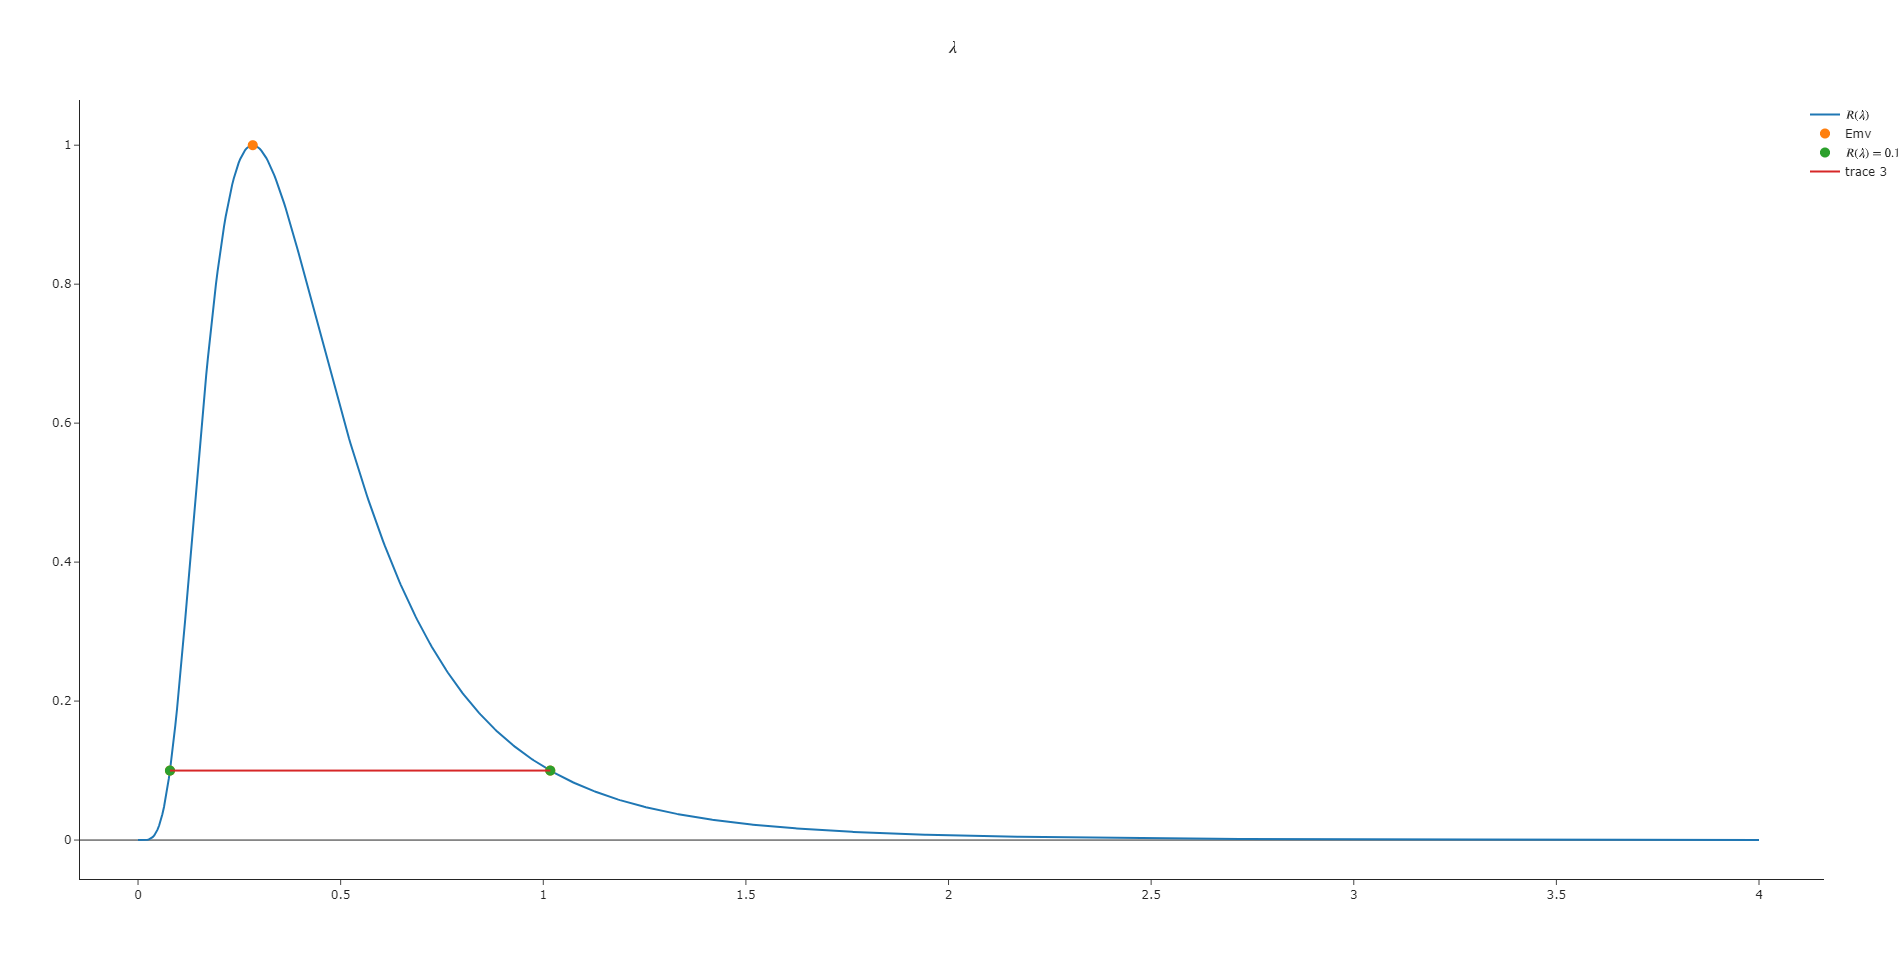
\includegraphics[scale=0.105]{Images/Int_ver.png}
				\end{center}
			\end{figure}

			No hay evidencia puesto que el invervalo de verosimilitud del $10\%$ de $\lambda$ no está completamente contenido dentro del intervalo $[0,1]$(podría pedir un mayor porcentaje pero tendriamos un mayor cesgo).
		\end{sol}
	\end{enumerate}
\end{document}

